\documentclass{article}


\usepackage[english]{babel}
\usepackage{listings}

\usepackage[letterpaper,top=2cm,bottom=2cm,left=3cm,right=3cm,marginparwidth=1.75cm]{geometry}

% Useful packages
\usepackage{amsmath}
\usepackage{graphicx}
\usepackage[colorlinks=true, allcolors=blue]{hyperref}
\usepackage{listings}
\lstset{language=Python}

\title{COSC 343: homework 2}
\author{Micah Sherry}

\begin{document}
\maketitle

\section{accelerated Newton's Method}
If the root $f(x) = 0$ is a double root (has multiplicity 2), then newtons method can be accelerated by using:
$$x_{n+1}= x_n - 2\frac{f(x)}{f^\prime(x_n)}$$
Numerically compare the convergence of this scheme with newtons method on a function with a known double root.
\\\\
For this question I will use the function: $f(x) = (x - 3)^2(1 + e^x)$ to compare the rate of convergence of Newton's Method and the Accelerated Newton's method.
\subsection*{code:}
\lstinputlisting{../fasterNewtonsMethod.py}
\subsection*{output and plots:}
	\begin{figure}[hbt!]
		\centering
		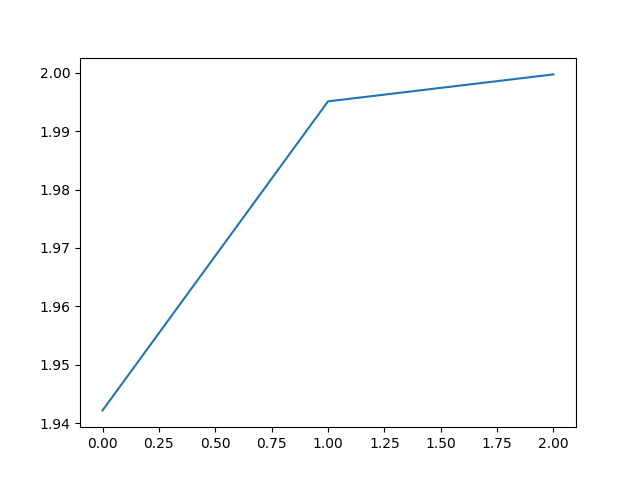
\includegraphics[width=.75\linewidth]{accelerated_alpha.png}
		\caption{accelerated newtons method}
		\label{fig: accelerated newtons method convergence}
	\end{figure}
	
	\begin{figure}[hbt!]
		\centering
		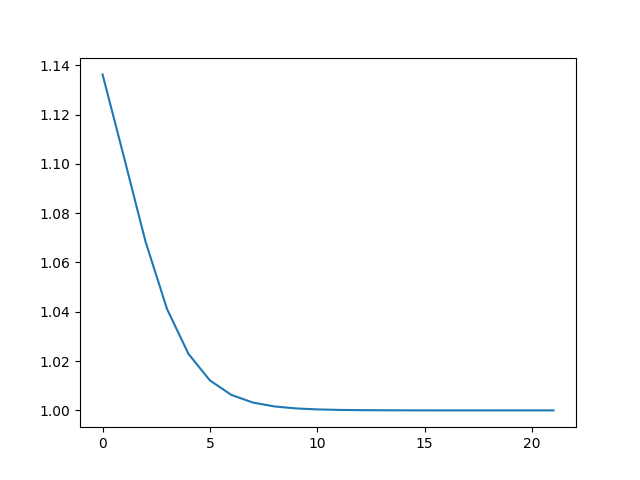
\includegraphics[width=.75\linewidth]{newtons_alpha.png}
		\caption{newtons method convergence}
		\label{fig: newtons method convergence}
	\end{figure}
Newton's method approximated the root of f(x) to be 3.000000071980329\\
Accelerated Newton's method approximated the root of f(x) to be 3.0 (not exactly 3.0)\\
From visual inspection of the graphs Newton's method converges at a rate of $O(h^1)$
and the accelerated Newton's method converges at a rate of $O(h^2)$. My hypothesis for why the accelerated Newton's method performs better than the standard Newton's method is that the two cancels out the two in the denominator that comes from the differentiating a squared term in the function. 
\pagebreak

\section{Newton's method with secant}
Write and test a recursive procedure for the secant method, Numerically estimate the methods order of convergence. Note in the secant method the derivative in Newton's method is replaced with an approximation 
$$f^\prime(x_i) \approx  \frac{f(x_i)-f(x_{i-1})}{x_i-x_{i-1}}$$
\\\\
for this question I will use the function $f(x) = (x - 4)(e^x + 1)$ to verify it works.


\subsection*{code:}
\lstinputlisting{../secantMethod.py}
\subsection*{output and plots:}
The secant method approximated the root of f(x) to be 4.000000000076314\\
From visual inspection of the graph (and discussion In class) we see that the secant method converges at a rate of approximately  $O(h^{1.6})$ or more accurately $O(h^{\phi})$ (where $\phi$ is the golden ratio)
	\begin{figure}[hbt!]
		\centering
		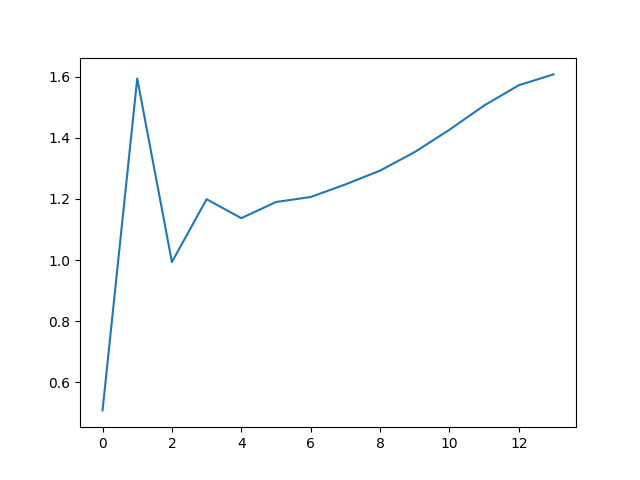
\includegraphics[width=.75\linewidth]{secant_alpha.png}
		\caption{secant method convergence}
		\label{fig: secant method convergence}
	\end{figure} 
	
	
\section{Olver's Method}
test numerically Olver's method given by
$$x_{n+1}= x_n - 2\frac{f(x_n)}{f^\prime(x_n)} - \frac{1}{2}\frac{f^{\prime\prime}(x_n)}{f^{\prime}(x_n)}\left[\frac{f(x_n)}{f^\prime(x_n)}\right]^2$$
establish an estimate for its rate of convergence.
\\\\
For Olver's I will use the function $f(x) = (x-3) * e^x$ to verify it works and find the rate of convergence
\subsection*{code:}
\lstinputlisting{../OlversMethod.py}
\subsection*{output and code}
Olver's method approximated the root of f(x) to be 3.000000000173341.\\
From inspection of the graph the rate of convergence appears to be $O(h^3)$. this makes since because Olver's method is derived from the three term expansion of Taylor's series which itself converges at a rate of  $O(h^3)$.
	\begin{figure}[hbt!]
		\centering
		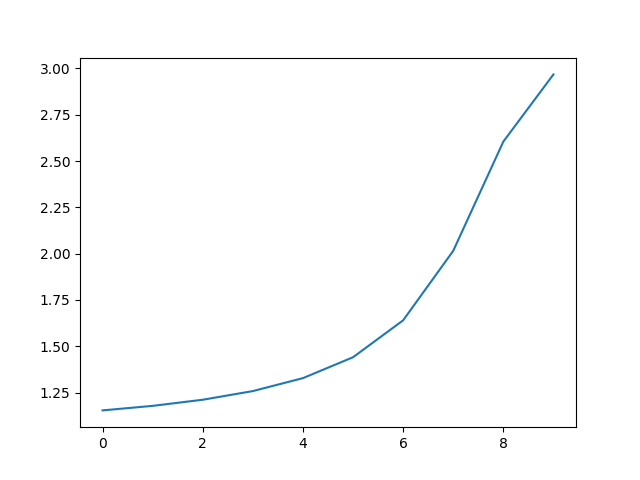
\includegraphics[width=.75\linewidth]{olvers_alpha.png}
		\caption{Olver's method convergence}
		\label{fig: Olver's method convergence}
	\end{figure} 
\pagebreak
\section{solving a Nonlinear system of equations}
write a program that can be used to solve the following non linear system
$$w_1 + w_2 = 2$$
$$w_1x_1 + w_2x_2 = 0$$
$$w_1x_1^2 + w_2x_2^2 = \frac{2}{3}$$
$$w_1x_1^3 + w_2x_2^3 = 0$$
how many different solutions can you find?\\
The first step I took to solve this system was to solve the system of equations was to solve each system for zero and assign each of them a function. 
$$f_0(x) = w_1 + w_2 - 2  $$
$$f_1(x) = w_1x_1 + w_2x_2 $$
$$f_2(x) = w_1x_1^2 + w_2x_2^2 - \frac{2}{3}  $$
$$f_3(x) = w_1x_1^3 + w_2x_2^3 $$
The next step was to find the Jacobian system for that I got

\renewcommand{\arraystretch}{1.5}  % Increase spacing by 1.5 times

$$\begin{pmatrix}
	1 & 1 & 0 & 0 \\
	x_1 & x_2 & w_1 & w_2 \\
	x_1^2 & x_2^2 & 2w_1 x_1 & 2w_2 x_2 \\
	x_1^3 & x_2^3 & 3w_1 x_1^2 & 3w_2 x_2^2
\end{pmatrix}$$
Then used Newton's method for vectors to find the root(s) of the system of equations
\subsection*{code:}
\lstinputlisting{../vectorNewtonsMethod.py}
\subsection*{solution}
The solutions are of the form $$\begin{bmatrix}
	w1\\
	w2\\
	x1\\
	x2
\end{bmatrix}$$
I was only able to find one solution to the system of equations.

$$\begin{bmatrix}
	1.0000 \\
	1.0000 \\
	0.5774 \\
	-0.5774 
\end{bmatrix}$$
\end{document}